

\chapter{IMPLEMENTATION}

\section{Methodology}

\hspace{0.9cm}The approach required for implementation of the proposed system would be an iterative model. The iterative process begins with a simple implementation of a subset of the software requirements and iteratively enhances versions until the entire system is implemented. The basic idea is to develop a system through repeated cycles and in small portions at a time.
This approach is suitable for the project because:
Modifications and improvements maybe required during the course of the life cycle.
Attempting to implement entire requirements at one go could prove risky. Smaller iterations will help eliminate issues at an earlier stage.
\begin{figure}[h!]
	\centering	
	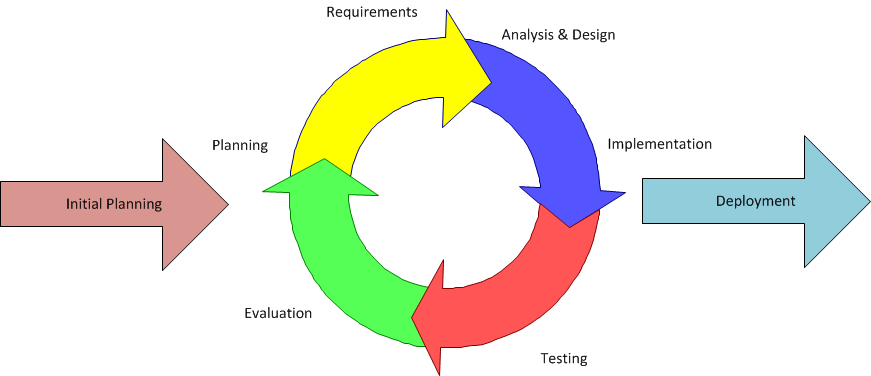
\includegraphics[width=5.5in]{iterative1.png} % e.g. insert ./image for image.png in the working directory, adjust scale as necessary
	\caption{Iterative Model of approach}
	\label{fig:1} % insert suitable label, this is used to refer to a fig from within the text as shown above
	
\end{figure} 

\section{Software}

\textbf{\hspace{0.9cm} Technologies Used} - 
	\begin{itemize}
	\item \textbf{GSM : } GSM is a TDMA based wireless
	network technology developed in Europe that is used
	throughout most of the world. Therefore in this project
	the GSM is the type of wireless that chooses. It is
	because it's the GSM is better than others wireless. It
	is suitable to install the systems that need a wide
	range. It also can monitor the signal strength and more
	adaptable. So it is suitable for our project. 
	\item \textbf{SMS : } Short message service is a mechanism
	of delivery of short messages over the mobile
	networks. It is a store and forward way of transmitting
	messages to and from mobiles.SMS supports national
	and international roaming. 
	\item \textbf{Android : }Android is a mobile operating
	platform owned by Google. Android is open source
	and Google releases the code under the Apache
	License. This open source code and permissive
	licensing allows the software to be freely modified
	and distributed by device manufacturers, wireless
	carriers and enthusiast developers. 
	\item \textbf{IDE Used : } Android Studio
\end{itemize}
\textbf{Why Android Studio? } The application is coded through the Android Studio IDE.
This is a comprehensive IDE for development of an
Android application with support on any OS and any
memory type(x64 / x86). This IDE is officially supported by Google and as such the higher popularity leads to better documentation and more available resources.
\newpage
\section{Design and Modeling}
\hspace{0.9cm} 
	\begin{itemize}
		\item \textbf{Design - } Based on the analysis of the system objectives and knowledge about various tools to be used, a rough system design is created. The different modules to be developed, the interaction between them, and their interaction with the system can be understood. The entire flow, beginning with login process to the hacker’s attempt is depicted.
		\begin{figure}[h!]
			\centering	
			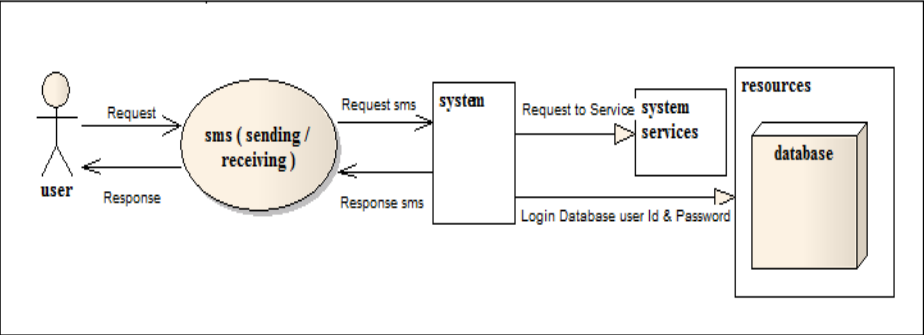
\includegraphics[width=5.5in]{sysarc.png} % e.g. insert ./image for image.png in the working directory, adjust scale as necessary
			\caption{System architecture diagram}
			\label{fig:2} % insert suitable label, this is used to refer to a fig from within the text as shown above
			
		\end{figure} 
		\end{itemize}
		
		
		\begin{figure}[h!]
		%	\centering	
			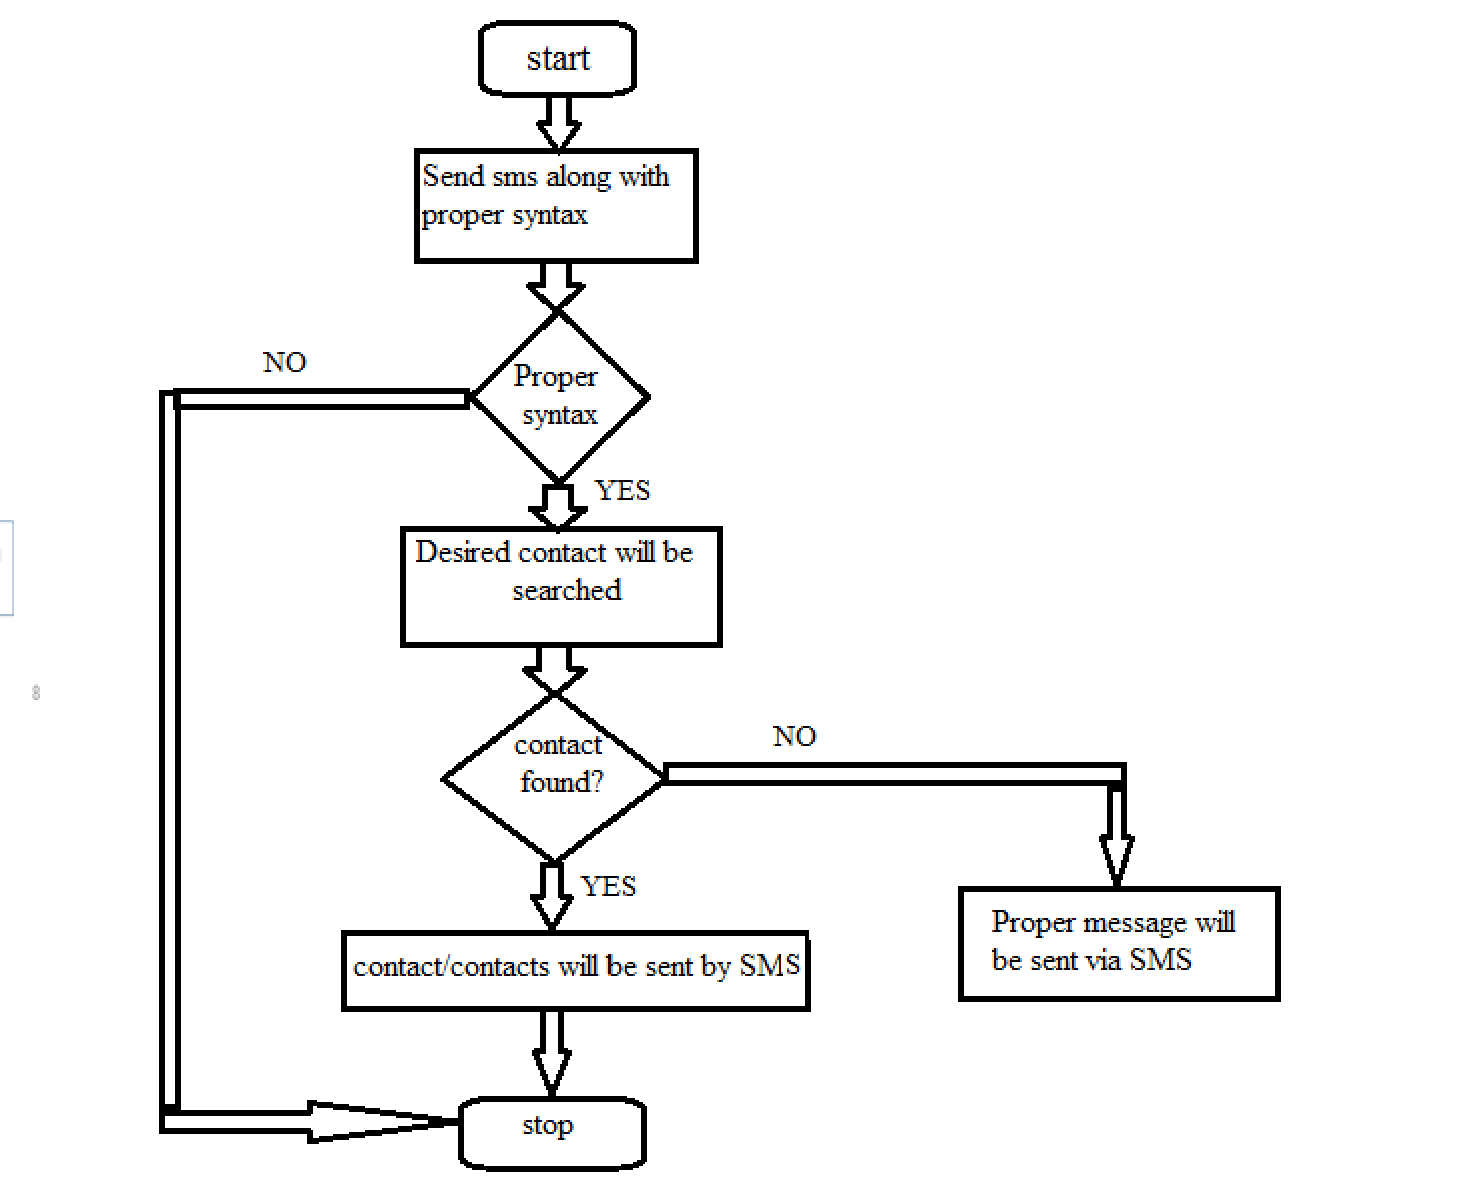
\includegraphics[width=5.5in]{workflow.png} % e.g. insert ./image for image.png in the working directory, adjust scale as necessary
			\caption{Work Flow diagram}
			\label{fig:3} % insert suitable label, this is used to refer to a fig from within the text as shown above
			
		\end{figure} 
	
	\begin{figure}[h!]
	%	\centering	
		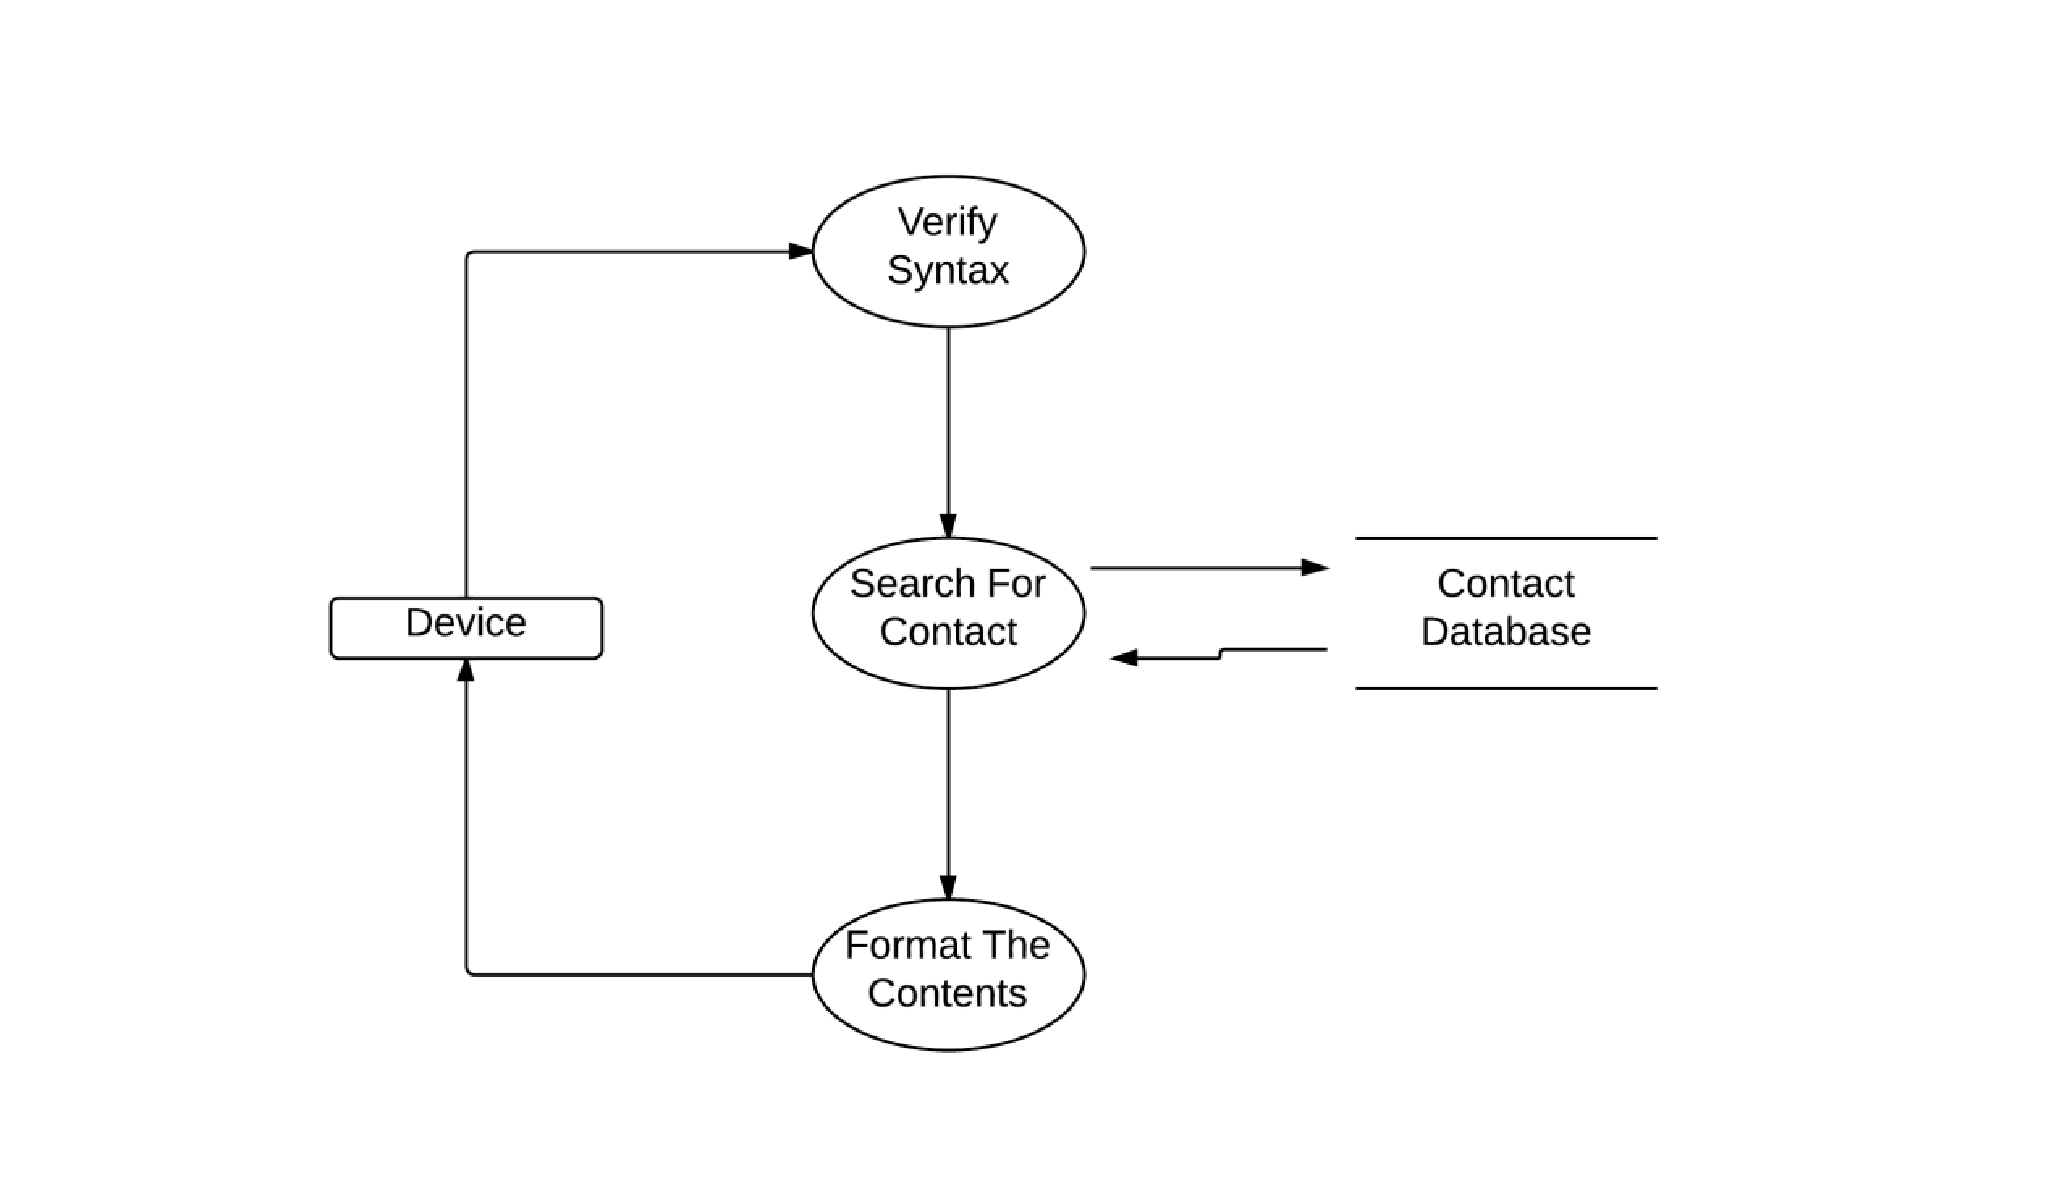
\includegraphics[width=5.5in]{dfd.png} % e.g. insert ./image for image.png in the working directory, adjust scale as necessary
		\caption{Data Flow Diagram}
		\label{fig:4} % insert suitable label, this is used to refer to a fig from within the text as shown above
		
	\end{figure} 

\begin{figure}[h!]
	%	\centering	
	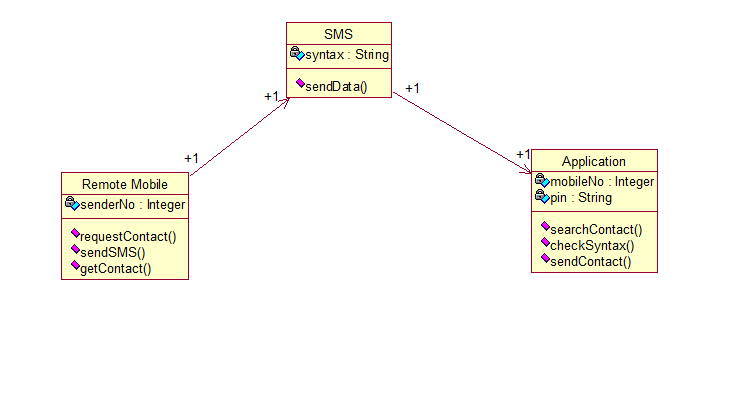
\includegraphics[width=5.5in]{class.png} % e.g. insert ./image for image.png in the working directory, adjust scale as necessary
	\caption{Class diagram}
	\label{fig:6} % insert suitable label, this is used to refer to a fig from within the text as shown above
	
\end{figure} 

	
	\begin{figure}[h!]
	%	\centering	
		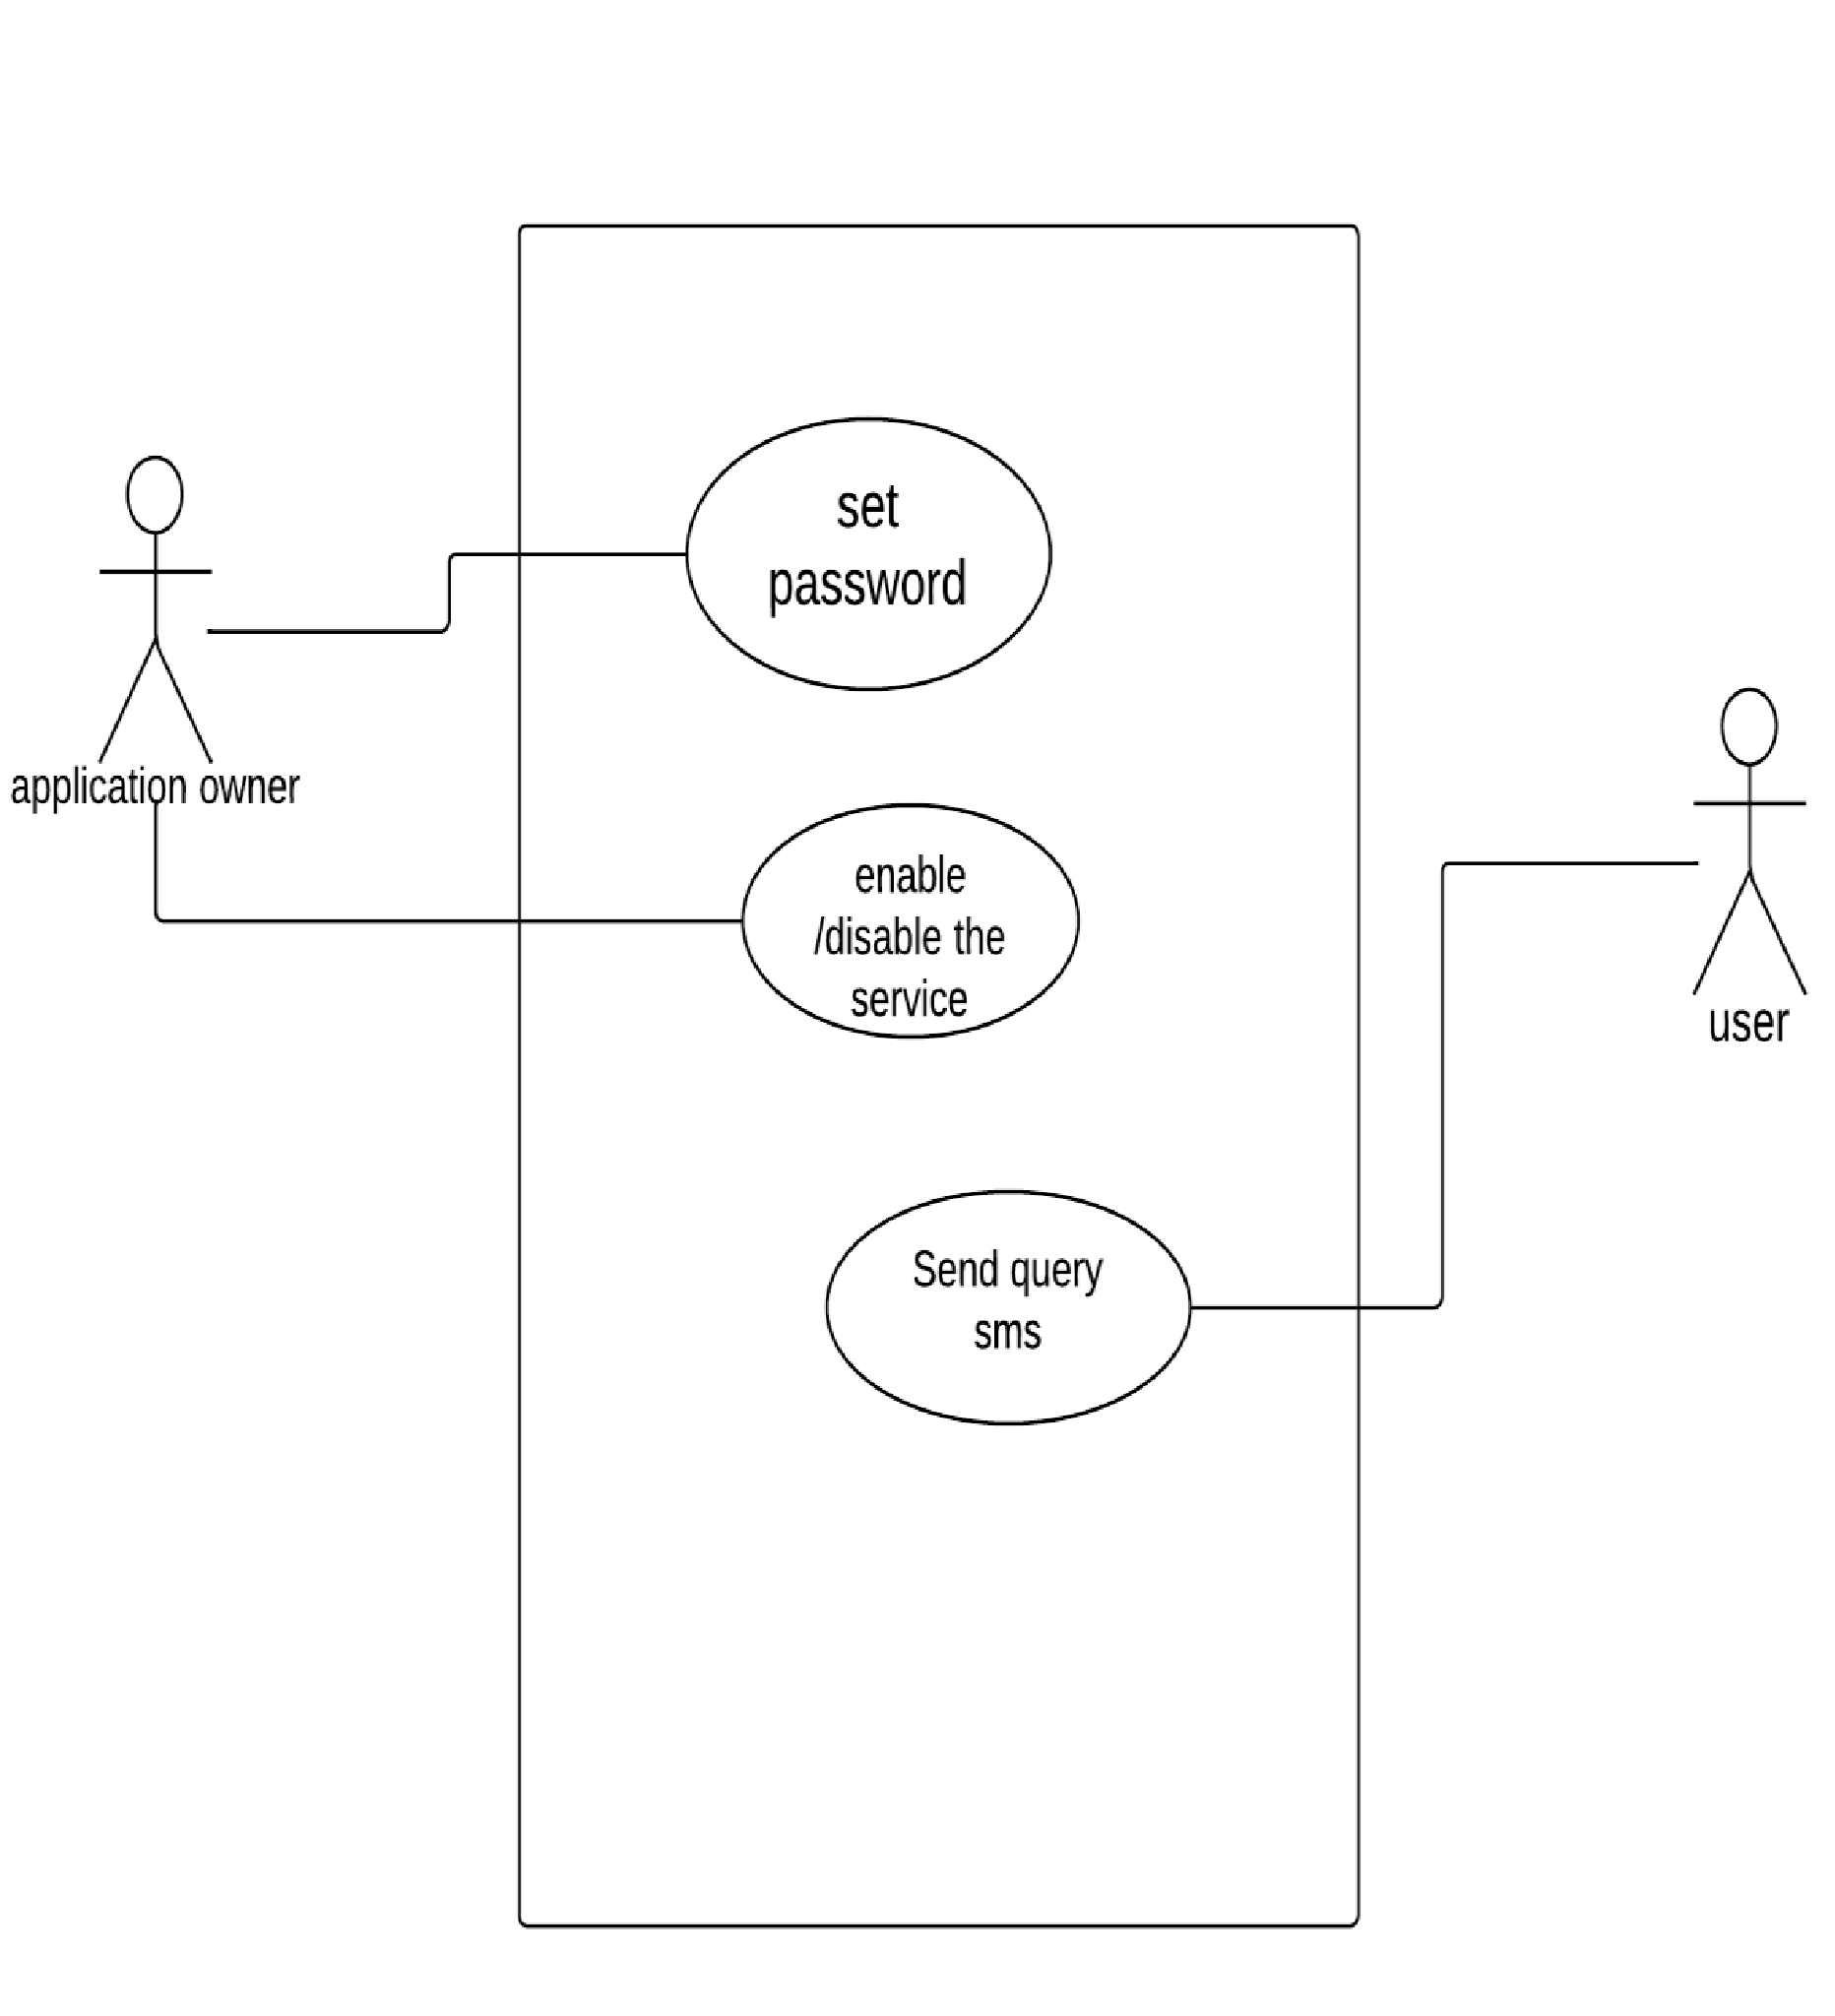
\includegraphics[width=5.5in]{usecase.png} % e.g. insert ./image for image.png in the working directory, adjust scale as necessary
		\caption{Use Case diagram}
		\label{fig:5} % insert suitable label, this is used to refer to a fig from within the text as shown above
		
	\end{figure} 

	 
	

	
	\begin{figure}[h!]
	%	\centering	
		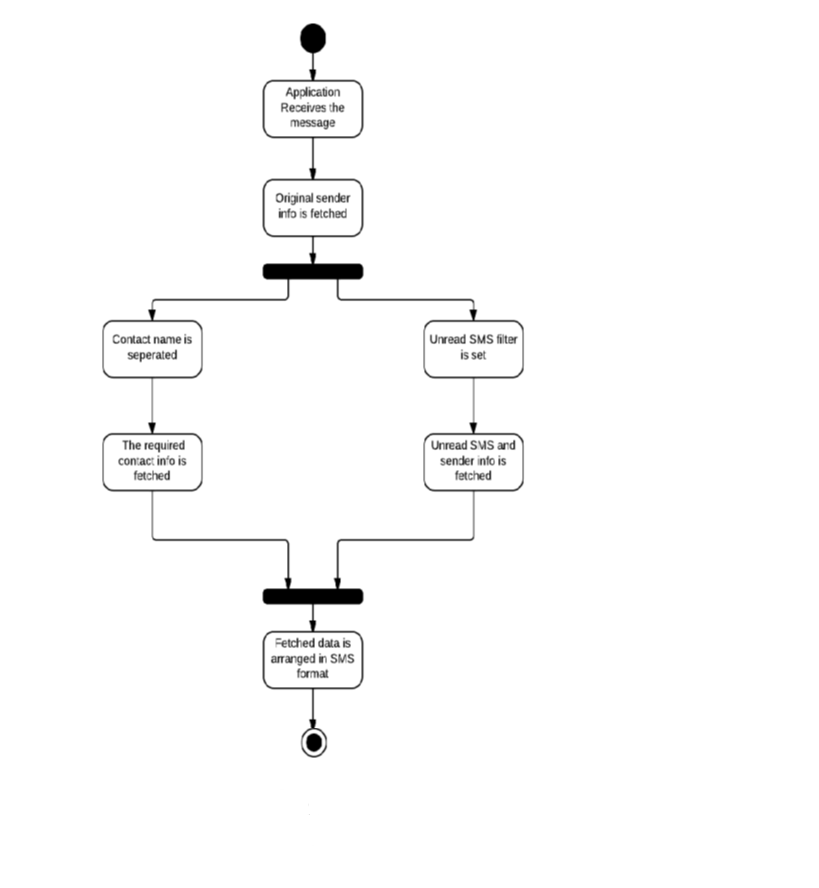
\includegraphics[width=5.5in]{activity.png} % e.g. insert ./image for image.png in the working directory, adjust scale as necessary
		\caption{Activity diagram}
		\label{fig:7} % insert suitable label, this is used to refer to a fig from within the text as shown above
		
	\end{figure} 

	 
	\begin{figure}[h!]
	%	\centering	
		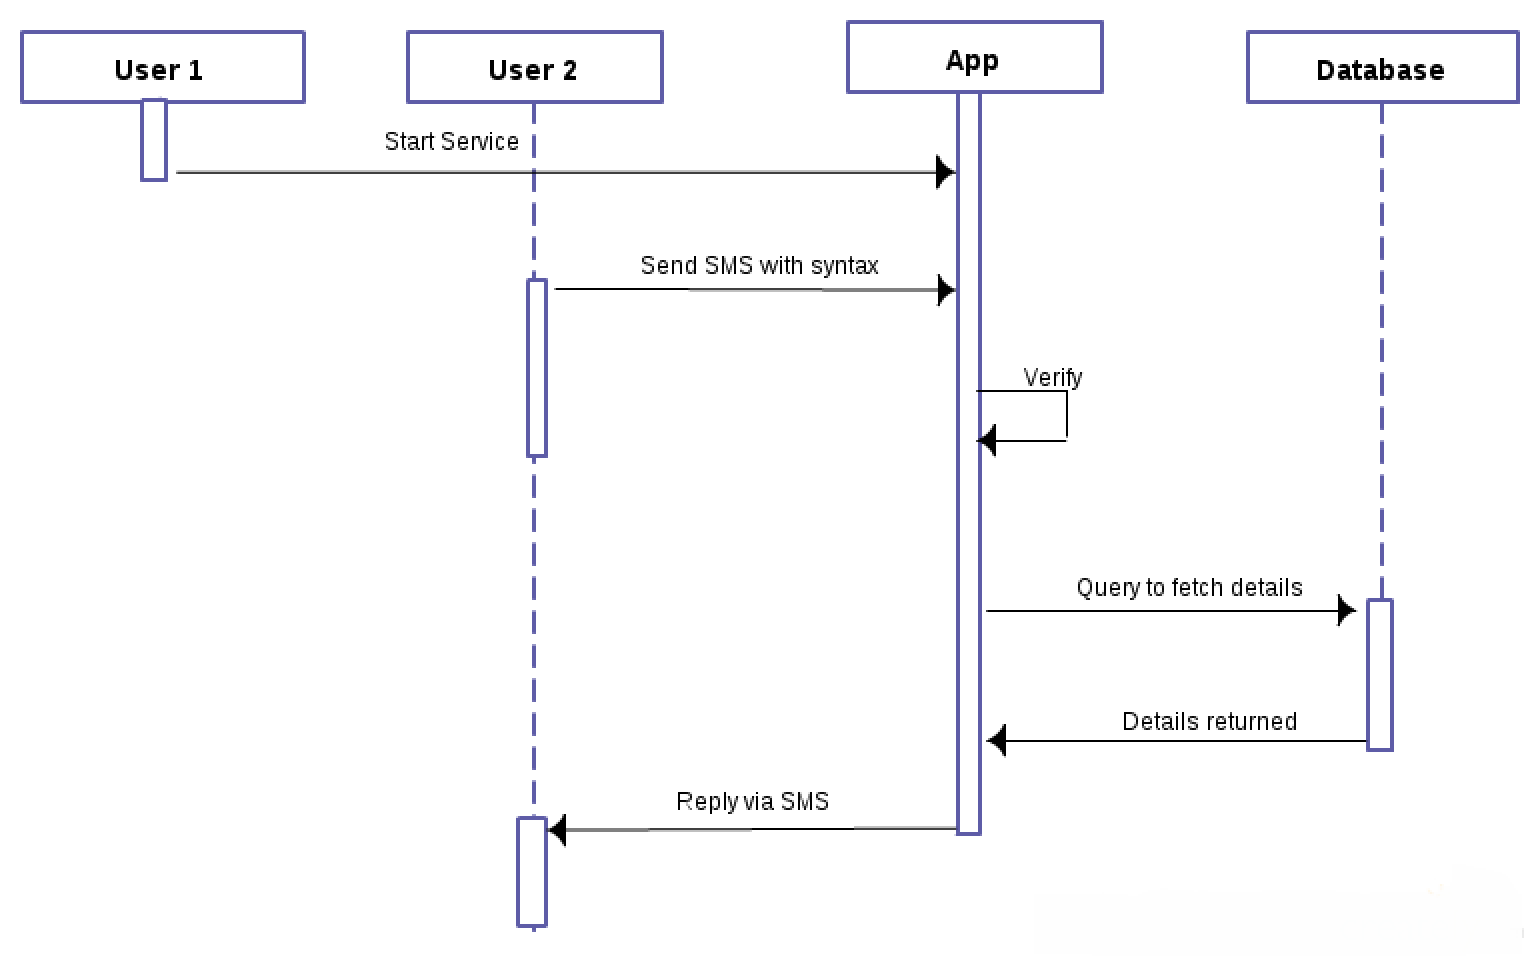
\includegraphics[width=5.5in]{sequence.png} % e.g. insert ./image for image.png in the working directory, adjust scale as necessary
		\caption{Sequence diagram}
		\label{fig:8} % insert suitable label, this is used to refer to a fig from within the text as shown above
		
	\end{figure} 
\newpage
\clearpage
\section{Implementation}

		\hspace{0.9cm}\paragraph{Code for Detecting received SMS:}
		\begin{verbatim}
	 public void onReceive(Context context, Intent intent) {
	
	Log.d("IYER","SMS Received");
	Toast.makeText(context, "SMS received", Toast.LENGTH_SHORT).show();
	
	if (intent.getAction() != null && (intent.getAction().equals(SMS_RECEIVED))) {
	
	// ---get the SMS message passed in---
	
	Bundle bundle = intent.getExtras();
	
	if (bundle != null) {
	
	// ---retrieve the SMS message received---
	
	Object[] pdus = (Object[]) bundle.get("pdus");
	
	for (int i = 0; i < pdus.length; i++) {
	
	//Need to check diff functions of SmsMesage  like getmsgbody works.
	SmsMessage currentMessage = SmsMessage.createFromPdu((byte[]) pdus[i]);
	
	String messageBody = currentMessage.getMessageBody();
	String phoneNumber = currentMessage.getOriginatingAddress();
	String displayMessageBody = currentMessage.getDisplayMessageBody();
	
	f1.check(context,phoneNumber,messageBody);
	
	} // end for loop
	}
	}
	}
	}
		\end{verbatim}
		
		\newpage
		\hspace{0.9cm}\paragraph{Code for Retreiving messages:}
		\begin{verbatim}
		 public void getAllSmsFromProvider() {
		List<String> lstSms = new ArrayList<String>();
		String s;
		ContentResolver cr = mcontext.getContentResolver();
		
		Cursor c = cr.query(Telephony.Sms.Inbox.CONTENT_URI, // Official CONTENT_URI 
		from docs
		new String[] {Telephony.Sms.Inbox.ADDRESS,
		Telephony.Sms.Inbox.BODY,  Telephony.Sms.Inbox.DATE_SENT }, // Select body text
		null,
		null,
		Telephony.Sms.Inbox.DEFAULT_SORT_ORDER); // Default sort order
		
		int totalSMS = 5;
		StringBuffer sb=new StringBuffer();
		
		if (c.moveToFirst()) {
		for (int i = 0; i < totalSMS; i++) {
		Date dateTime = new Date(Long.valueOf(c.getString(2)));
		s="No-"+c.getString(0)+",Text-"+c.getString(1)+",Date-"+dateTime;
		c.moveToNext();
		Log.d("IYER",s);
		sb.append(s);
		
		}
		sendSMS(phNO,sb.toString());
		} else {
		sendSMS(phNO,"No messages found");
		}
		c.close();
		
		
		}
		
		\end{verbatim}
		\newpage
			\hspace{0.9cm}\paragraph{Code for Retreiving calllog:}\cite{citation-7}
		\begin{verbatim}
		    public void calllog(String phoneNumber, String messageBody, 
		    String password,Context context) {
		
		 StringBuffer sb= new StringBuffer();
		
		ContentResolver c= context.getContentResolver();
		Cursor cursor=c.query(CallLog.Calls.CONTENT_URI,null,null,null,null);
		int i;
		sb.append("CALL LOGs \n");
		
		for(i=0;i<5;i++) {
			while (cursor.moveToNext()) {
				String phNumber = cursor.getString(cursor.getColumnIndex(CallLog.Calls.NUMBER));
				String callType = cursor.getString(cursor.getColumnIndex(CallLog.Calls.TYPE));
				String callDate = cursor.getString(cursor.getColumnIndex(CallLog.Calls.DATE));
				
				Date callDayTime = new Date(Long.valueOf(callDate));
				
				if (Integer.parseInt(callType) == CallLog.Calls.INCOMING_TYPE ||
				 Integer.parseInt(callType) == CallLog.Calls.MISSED_TYPE || Integer.parseInt(callType) ==
				  CallLog.Calls.OUTGOING_TYPE) {
					sb.append("\n Phone Number: " + phNumber + "   Call Date: " + callDayTime);
				}
				
			}
		}
		\end{verbatim}
		
		\newpage
		\hspace{0.9cm}\paragraph{Code for Retreiving contact:}\cite{citation-5}
		\begin{verbatim}
		 public void contacts(String phoneNumber,String messageBody, String password, 
		 Context context)
		{
		StringBuffer sb=new StringBuffer();
		ContentResolver c=context.getContentResolver();
		Cursor cursor=c.query(ContactsContract.Contacts.CONTENT_URI,null,null,null,null);
		String substr=messageBody.substring(messageBody.indexOf("getcontact"));
		
		String[] separated = substr.split(",");
		StringBuffer con=new StringBuffer();
		int i;
		
		while(cursor.moveToNext()){
		String id=cursor.getString(cursor.getColumnIndex(ContactsContract.Contacts._ID));
		String name=cursor.getString(cursor.getColumnIndex(
		ContactsContract.Contacts.DISPLAY_NAME));
		
		if(!messageBody.toLowerCase().contains(name.toLowerCase()))
		{
		continue;
		}
		
		Cursor pcursor=c.query(ContactsContract.CommonDataKinds.Phone.CONTENT_URI,null,
		ContactsContract.CommonDataKinds.Phone.CONTACT_ID+"=?",new String[]{id},null);
		
		while (pcursor.moveToNext()){
		String number=pcursor.getString(pcursor.getColumnIndex(
		ContactsContract.CommonDataKinds.Phone.NUMBER));
		sb.append(name+":"+number+",");
		}
		pcursor.close();
		}
		Log.d("IYER","contactsflasg");
		Toast.makeText(context, sb.toString(), Toast.LENGTH_SHORT).show();
		sendSMS(phoneNumber,sb.toString());
		cursor.close();
		}
		
		\end{verbatim}
		
		
			
		\hspace{0.9cm}\paragraph{Code for Retreiving location:}\cite{citation-6}
		\begin{verbatim}
		
		public void locate(Context context, String phoneNumber) {
			Toast.makeText(context, "Locating", Toast.LENGTH_SHORT).show();
			Log.d("IYER", "Locating");
			GoogleApiClient.Builder builder=new GoogleApiClient.Builder(
			context.getApplicationContext());
			builder.addApi(LocationServices.API);
			builder.addConnectionCallbacks(this);
			builder.addOnConnectionFailedListener(this);
			mLocationClient=builder.build();
			if (mLocationClient != null) {
				mLocationClient.connect();
			}
			
		}
		
		
		@Override
		public void onConnected(Bundle bundle) {
			String address="";
			mLastLocation=LocationServices.FusedLocationApi.getLastLocation(mLocationClient);
			
			if(mLastLocation!=null){
				double latitude=mLastLocation.getLatitude();
				double longitude=mLastLocation.getLongitude();
				
				
				Geocoder geocoder=new Geocoder(mcontext.getApplicationContext(), Locale.ENGLISH);
				try{
					List<android.location.Address> addresses=geocoder.getFromLocation(latitude,
					longitude,1);
					if(addresses!=null){
						android.location.Address fetchedAddress= addresses.get(0);
						address="i am at: "+fetchedAddress.getFeatureName()+","
						+fetchedAddress.getSubLocality()+","
						+fetchedAddress.getLocality()+"-"+fetchedAddress.getPostalCode()+","
						+fetchedAddress.getAdminArea()
						+","+fetchedAddress.getCountryName();
						
					}
				}
				catch (Exception e){
					e.printStackTrace();
				}
				/*
				sendSMS(phNO,address.toString());
				*/
				
				sendSMS(phNO,"http://maps.google.com/?q="+latitude+","
				+longitude+" "+address.toString());
				
			}
			else {
				address="Location not found";
			}
			
		}
		\end{verbatim}
		\newpage
		\section{GUI}
			\begin{figure}[h!]
				\centering	
			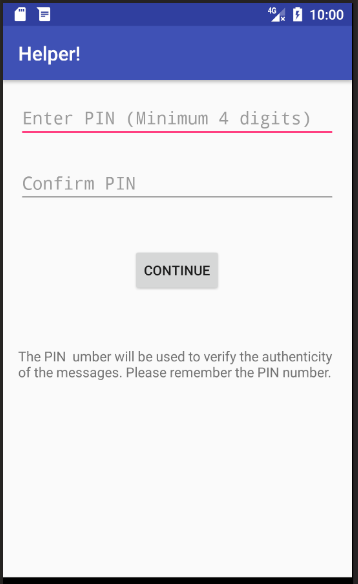
\includegraphics[scale=0.8]{1.png} % e.g. insert ./image for image.png in the working directory, adjust scale as necessary
			\caption{Initial screen on 1st usage}
			\label{fig:8} % insert suitable label, this is used to refer to a fig from within the text as shown above
			
		\end{figure} 
	
		\begin{figure}[h!]
			\centering	
		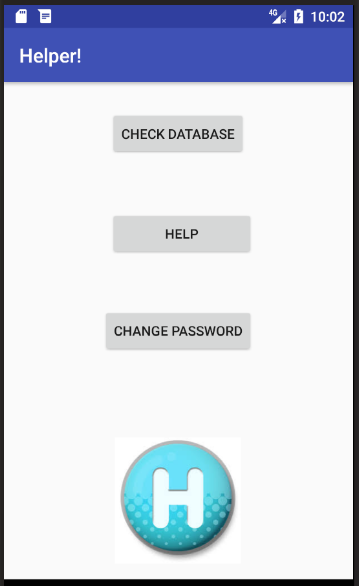
\includegraphics[scale=0.8]{2.png} % e.g. insert ./image for image.png in the working directory, adjust scale as necessary
		\caption{Home screen}
		\label{fig:8} % insert suitable label, this is used to refer to a fig from within the text as shown above
		
		\end{figure} 

			\begin{figure}[h!]
				\centering	
			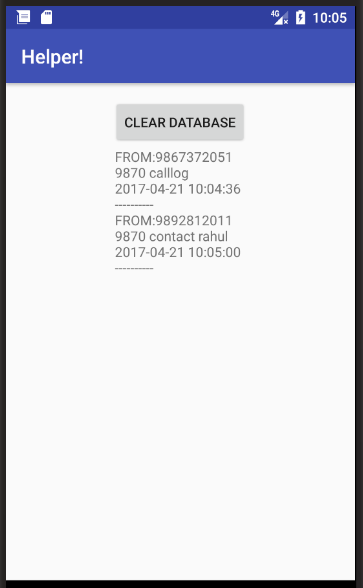
\includegraphics[scale=0.8]{3.png} % e.g. insert ./image for image.png in the working directory, adjust scale as necessary
			\caption{Database}
			\label{fig:8} % insert suitable label, this is used to refer to a fig from within the text as shown above
			
		\end{figure} 
	
			\begin{figure}[h!]
			\centering	
			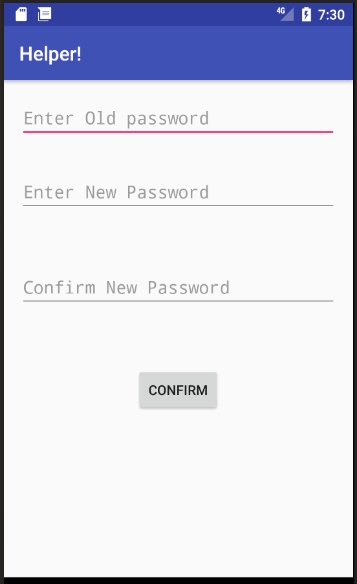
\includegraphics[scale=0.8]{4.png} % e.g. insert ./image for image.png in the working directory, adjust scale as necessary
			\caption{Change Password}
			\label{fig:8} % insert suitable label, this is used to refer to a fig from within the text as shown above
			
		\end{figure} 
		
		
		
		


